\chapter{Security}
\url{https://docs.microsoft.com/en-us/previous-versions/windows/it-pro/windows-server-2008-r2-and-2008/cc772066(v=ws.10)}

\section{User Account Control (UAC)}
\label{windows_knowledge:fundamentals:security:uac}

\href{https://docs.microsoft.com/en-us/windows/security/identity-protection/user-account-control/how-user-account-control-works}{User
Account Control (UAC)}~\ref{windows_knowledge:ad:rights_privileges:uac}
 is used to allow an administrator user to not give administrator privileges to each process executed. This is achieved using default the low privileged token of the user. When, the administrator executes some process as administrator, a UAC elevation is performed and if it is successfully completed, the privileged token is used to create the process.

To differentiate which process is executed with low or high privileges
\emph{Mandatory Integrity Controls (MIC)} are used.

Some programs are autoelevated automatically if the user belongs to the administrator group. These binaries have inside their Manifests the autoElevate option with value True. The binary has to be signed by Microsoft also.

Then, to bypass the UAC (elevate from medium integrity level to high) some
attackers use this kind of binaries to execute arbitrary code because it will
be executed from a High level integrity processi.

\verb+sigcheck.exe+ from Sysinternals allow to check the Manifest of a binary


The following diagram, adapted from the source here, illustrates how UAC works.

\begin{figure}
  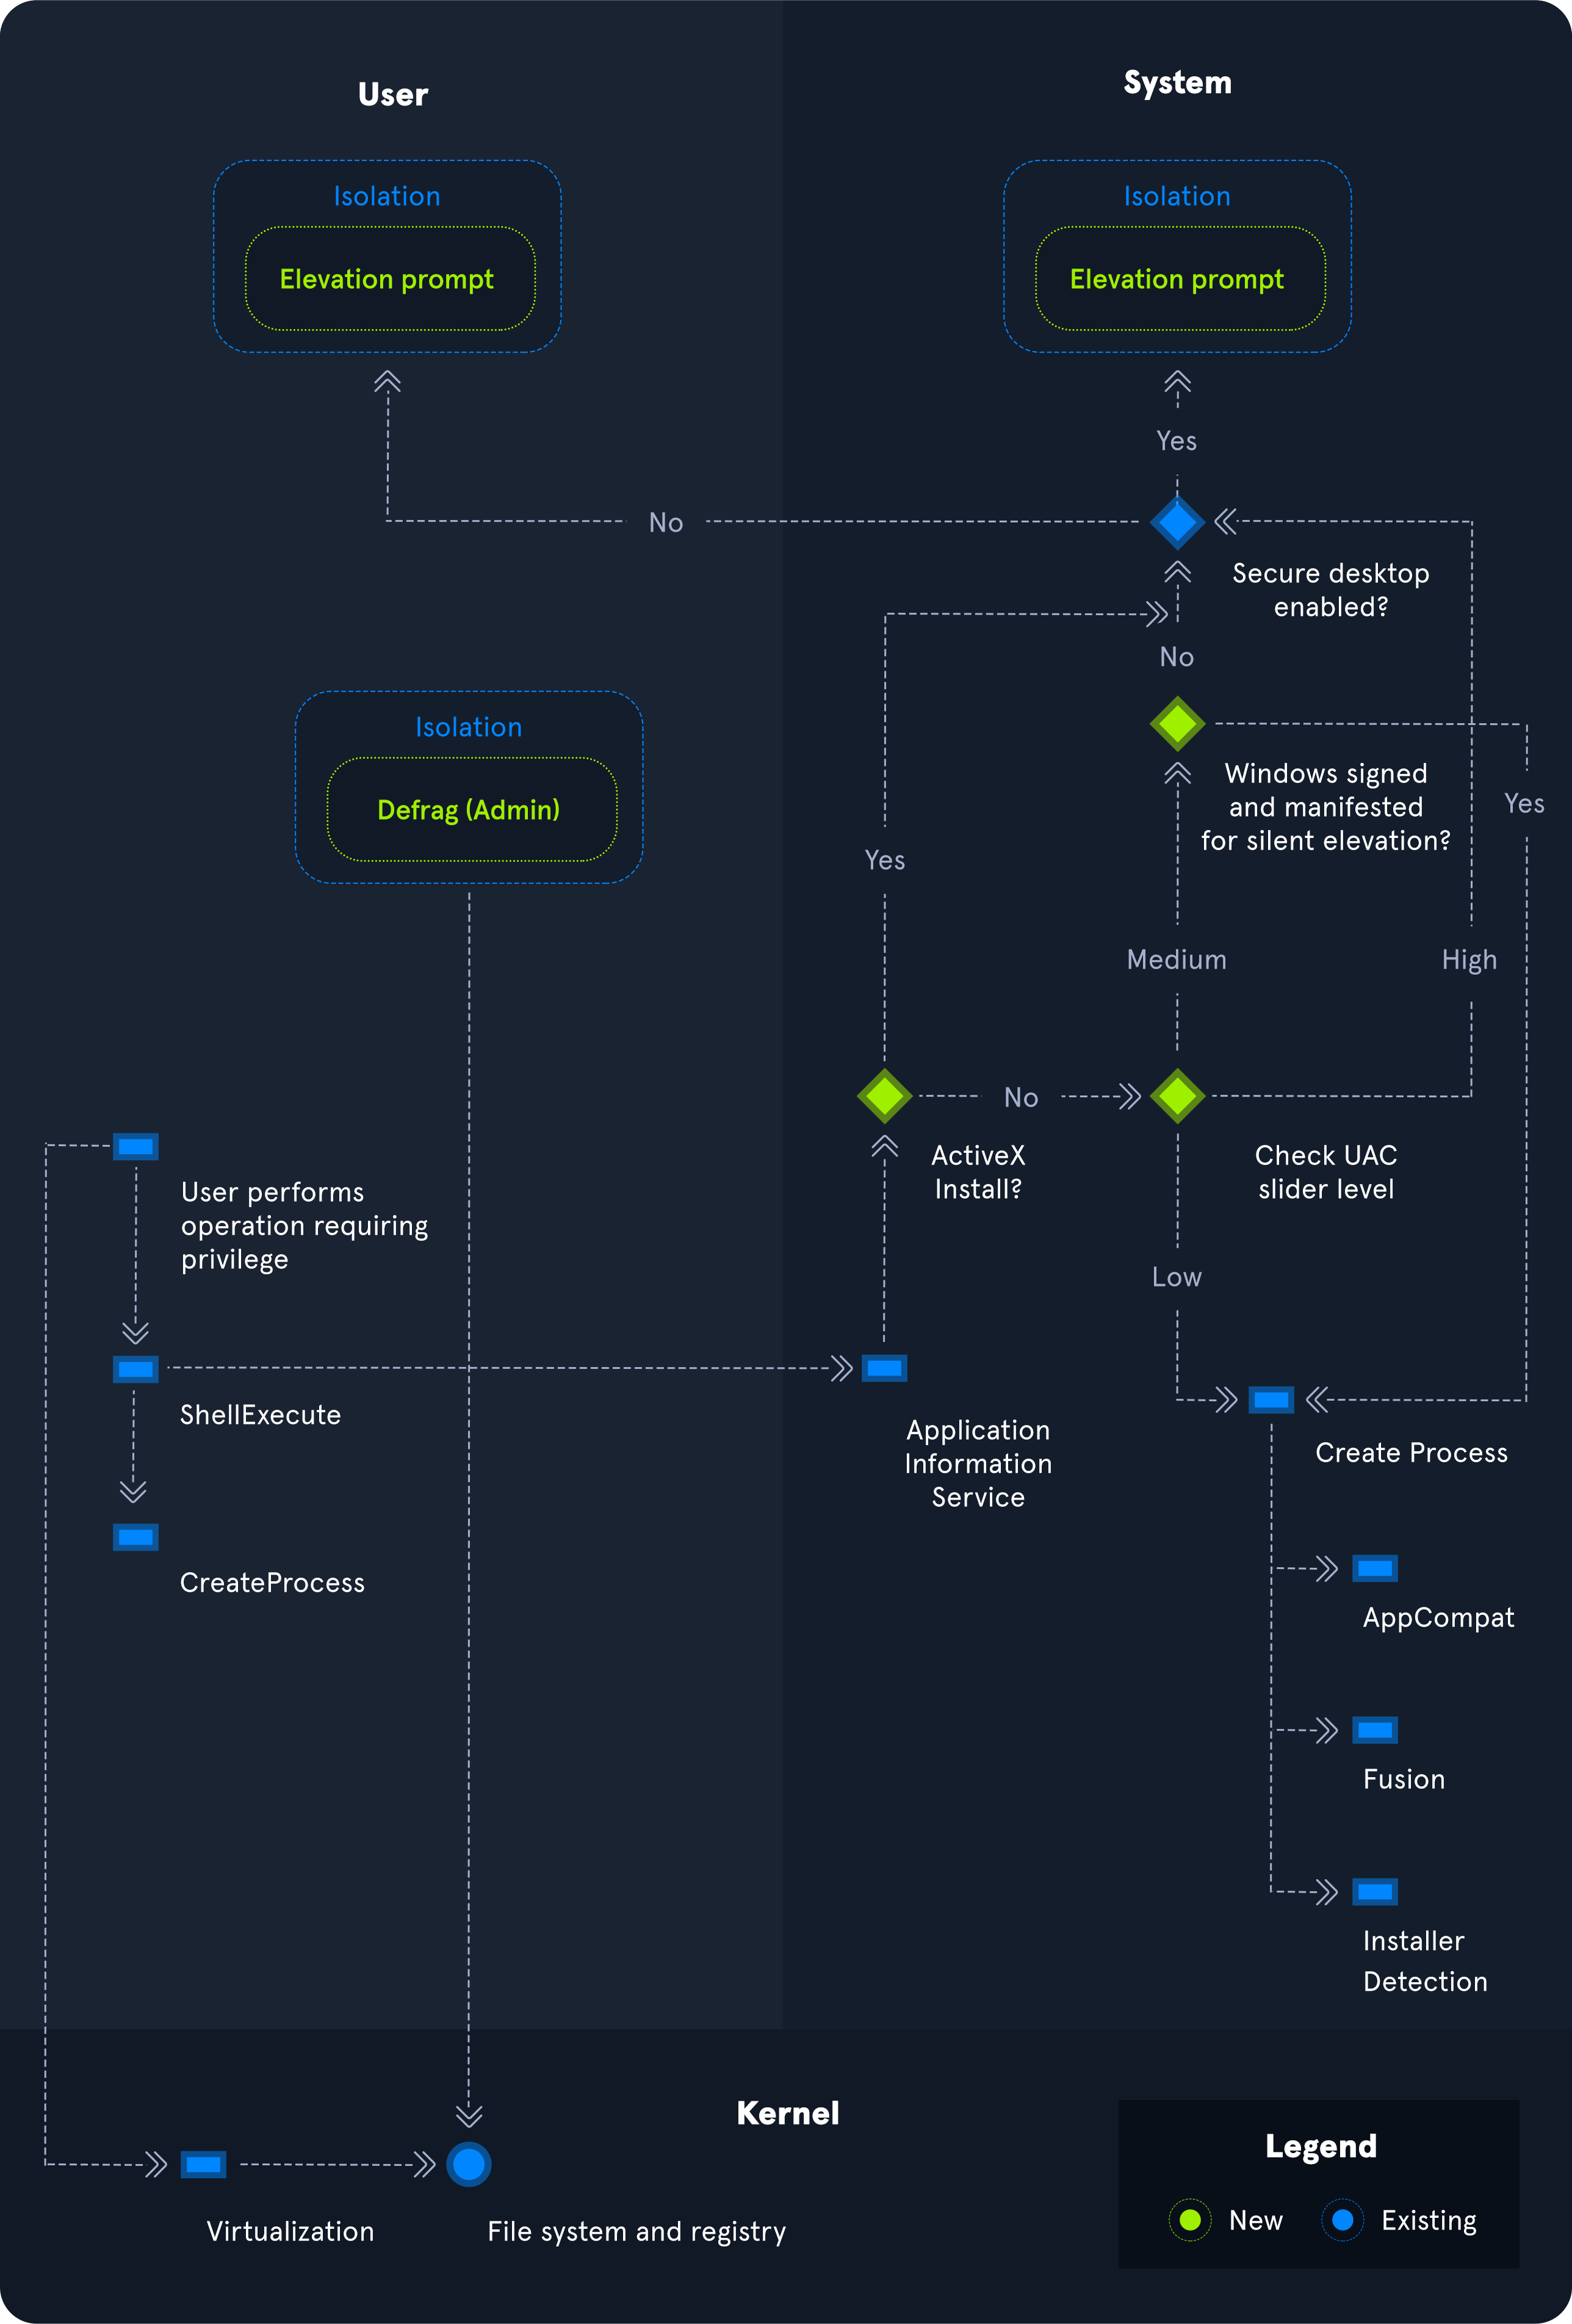
\includegraphics[width=\linewidth]{windows_knowledge/security/images/uac_architecture.png}
  \caption{UAC architecture}
  \label{fig:uac-architecture}
\end{figure}

\section{Registry}
\index{Windows!registry}
\label{win:registry}

The \href{https://en.wikipedia.org/wiki/Windows_Registry}{Registry} is a
hierarchical database in Windows critical for the operating system. It stores
low-level settings for the Windows operating system and applications that
choose to use it. It is divided into computer-specific and user-specific data.


The \verb+regedit+ command allow to view/edit it.

The tree-structure consists of main folders (root keys) in which subfolders
(subkeys) with their entries/files (values) are located. There are 11 different
types of values that can be entered in a subkey.

Each folder under i\verb+Computer+ is a key. The root keys all start with
\verb+HKEY+. A key such as \verb+HKEY-LOCAL-MACHINE+ is abbreviated to
i\verb+HKLM+. 

\verb+HKLM+ contains all settings that are relevant to the local system. This
root key contains six subkeys like \verb+SAM+, \verb+SECURITY+, \verb+SYSTEM+,
\verb+SOFTWARE+, \verb+HARDWARE+, and \verb+BCD+, loaded into memory at boot
time (except HARDWARE which is dynamically loaded).

The entire system registry is stored in several files on the operating system.
You can find these under \verb+C:\Windows\System32\Config\+.

The user-specific registry hive (\verb+HKCU+) is stored in the user folder
(i.e., \verb+C:\Windows\Users\<USERNAME>\Ntuser.dat+).

\section{Run and RunOnce Registry Keys}

There are also so-called \gls{win:registry-hive}, which contain a logical group
of keys, subkeys, and values to support software and files loaded into memory
when the operating system is started or a user logs in. These hives are useful
for maintaining access to the system. These are called
\href{https://docs.microsoft.com/en-us/windows/win32/setupapi/run-and-runonce-registry-keys}{Run
and RunOnce registry keys}.

\section{AppLocker (Application Whitelisting)}
\label{windowd_knowledge:fundamentals:security:applocker}
An application whitelist is a list of approved software applications or executables allowed to be present and run on a system. The goal is to protect the environment from harmful malware and unapproved software that does not align with the specific business needs of an organization. Implementing an enforced whitelist can be a challenge, especially in a large network. An organization should implement a whitelist in audit mode initially to make sure that all necessary applications are whitelisted and not blocked by an error of omission, which can cause more problems than it fixes.

Blacklisting, in contrast, specifies a list of harmful or disallowed software/applications to block, and all others are allowed to run/be installed. Whitelisting is based on a "zero trust" principle in which all software/applications are deemed "bad" except for those specifically allowed. Maintaining a whitelist generally has less overheard as a system administrator will only need to specify what is allowed and not constantly update a "blacklist" with new malicious applications.

Whitelisting is recommended by organizations such as NIST, especially in high-security environments.

\href{https://docs.microsoft.com/en-us/windows/security/threat-protection/windows-defender-application-control/applocker/applocker-overview}{AppLocker} is Microsoft's application whitelisting solution and was first introduced in Windows 7. AppLocker gives system administrators control over which applications and files users can run. It gives granular control over executables, scripts, Windows installer files, DLLs, packaged apps, and packed app installers.

It allows for creating rules based on file attributes such as the publisher's name (which can be derived from the digital signature), product name, file name, and version. Rules can also be set up based on file paths and hashes. Rules can be applied to either security groups or individual users, based on the business need. AppLocker can be deployed in audit mode first to test the impact before enforcing all of the rules.


\section{Local Group Policy}
Group Policy allows administrators to set, configure, and adjust a variety of settings. In a domain environment, group policies are pushed down from a Domain Controller onto all domain-joined machines that Group Policy objects (GPOs) are linked to. These settings can also be defined on individual machines using Local Group Policy.

Group Policy can be configured locally, in both domain environments and non-domain environments. Local Group Policy can be used to tweak certain graphical and network settings that are otherwise not accessible via the Control Panel. It can also be used to lock down an individual computer policy with stringent security settings, such as only allowing certain programs to be installed/run or enforcing strict user account password requirements.

We can open the Local Group Policy Editor by opening the Start menu and typing
\verb+gpedit.msc+. The editor is split into two categories under Local Computer
Policy - \emph{Computer Configuration} and \emph{User Configuration}.

 
Local Group Policy Editor enables fine-tuned account auditing and configure
AppLocker.

\section{Microsoft Defender}
\label{windowd_knowledge:fundamentals:security:defender}
\href{https://en.wikipedia.org/wiki/Microsoft_Defender}{Microsoft Defender}, formerly known as Windows Defender, is built-in antivirus that ships for free with Windows operating systems. It was first released as a downloadable anti-spyware tool for Windows XP and Server 2003. Defender started coming prepackaged as part of the operating system with Windows Vista/Server 2008. The program was renamed to Windows Defender Antivirus with the Windows 10 Creators Update.

Defender comes with several features such as real-time protection, which protects the device from known threats in real-time and cloud-delivered protection, which works in conjunction with automatic sample submission to upload suspicious files for analysis. When files are submitted to the cloud protection service, they are "locked" to prevent any potentially malicious behavior until the analysis is complete. Another feature is Tamper Protection, which prevents security settings from being changed through the Registry, PowerShell cmdlets, or group policy.

Windows Defender is managed from the Security Center, from which a variety of additional security features and settings can be enabled and managed.

Real-time protection settings can be tweaked to add files, folders, and memory areas to controlled folder access to prevent unauthorized changes. We can also add files or folders to an exclusion list, so they are not scanned. An example would be excluding a folder of tools used for penetration testing from scanning as they will be flagged malicious and quarantined or removed from the system. Controlled folder access is Defender's built-in Ransomware protection.

We can use the PowerShell cmdlet \verb+Get-MpComputerStatus+ to check which protection settings are enabled.

Windows Defender is not without its flaws and should be part of a defense-in-depth strategy built around core principles of configuration and patch management, not treated as a silver bullet for protecting our systems. Definitions are updated constantly, and new versions of Windows Defender are built-in to major operating releases such as Windows 10, version 1909, which is the most recent version at the time of writing.

Windows Defender will pick up payloads from common open-source frameworks such as Metasploit or unaltered versions of tools such as Mimikatz.

\section{BitLocker}

